\documentclass[border=12pt]{standalone}
\usepackage{tikz}
\usetikzlibrary{arrows.meta,backgrounds,fit}
\usepackage[T1]{fontenc}
\usepackage[scaled=0.95]{helvet}
\renewcommand{\familydefault}{\sfdefault}
\usepackage{xcolor}

\definecolor{accent}{RGB}{43,100,170}
\definecolor{accentlight}{RGB}{240,246,255}
\definecolor{accentmid}{RGB}{43,100,170}
\definecolor{specgreen}{RGB}{22,120,60}
\definecolor{specgreenlight}{RGB}{218,250,232}
\definecolor{analysisbg}{RGB}{247,248,250}

\begin{document}
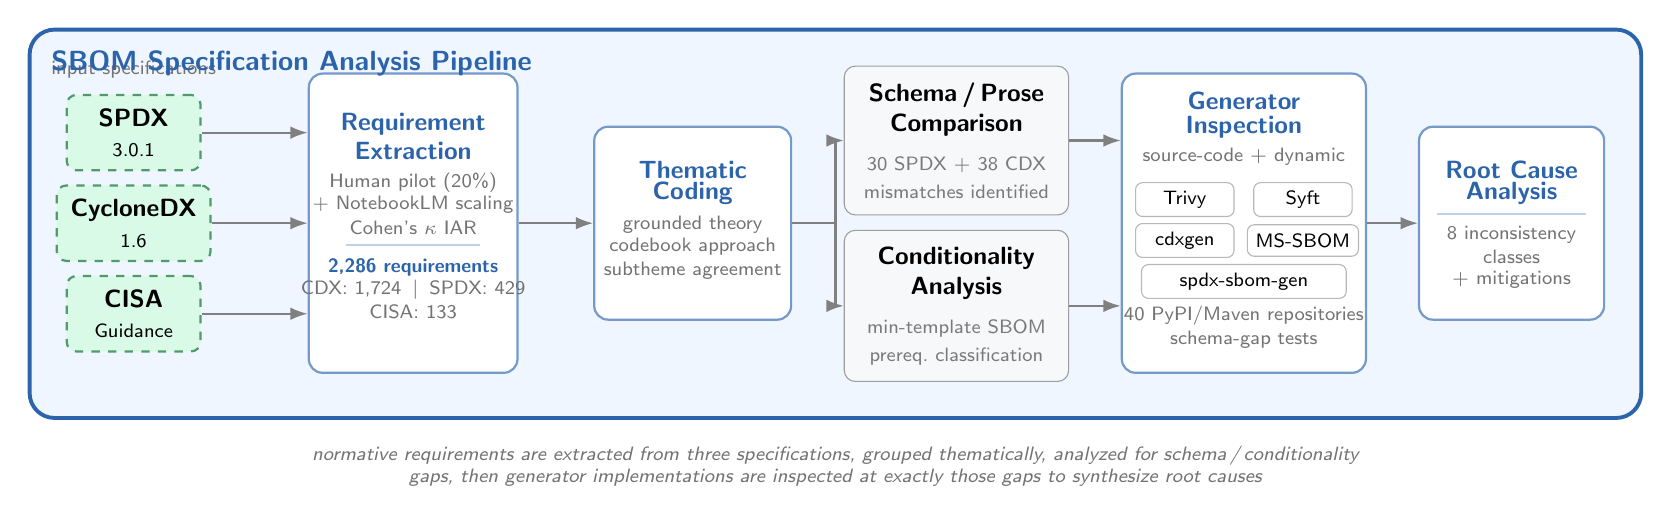
\begin{tikzpicture}[
  font=\sffamily,
  arr/.style={-{Latex[length=2.2mm,width=1.6mm]}, line width=0.75pt, color=black!50},
  specbox/.style={
    draw=specgreen!75, fill=specgreenlight,
    rounded corners=3.5pt, dashed, thick,
    inner sep=5pt, align=center,
    minimum width=1.7cm, minimum height=0.78cm,
    font=\small\sffamily
  },
  stagebox/.style={
    draw=accent!65, fill=white,
    rounded corners=5pt, thick,
    inner sep=8pt, align=center,
    font=\small\sffamily
  },
  analysisbox/.style={
    draw=black!38, fill=analysisbg,
    rounded corners=4pt,
    inner sep=6pt, align=center,
    minimum width=2.85cm, minimum height=1.6cm,
    font=\small\sffamily
  },
  toolchip/.style={
    draw=black!28, fill=white,
    rounded corners=2.5pt,
    inner sep=3pt, align=center,
    minimum width=1.25cm, minimum height=0.4cm,
    font=\scriptsize\sffamily
  },
  sublabel/.style={font=\scriptsize\sffamily, text=black!55},
  boldlabel/.style={font=\small\bfseries\sffamily, text=accent}
]

%% ─────────────────────────────────────────────────────────────────────────────
%% Stage 0 : Input Specifications
%% ─────────────────────────────────────────────────────────────────────────────
\node[sublabel, anchor=south] at (0, 1.72) {input specifications};
\node[specbox] (spdx) at (0,  1.15) {\textbf{SPDX}\\\scriptsize 3.0.1};
\node[specbox] (cdx)  at (0,  0.00) {\textbf{CycloneDX}\\\scriptsize 1.6};
\node[specbox] (cisa) at (0, -1.15) {\textbf{CISA}\\\scriptsize Guidance};

%% ─────────────────────────────────────────────────────────────────────────────
%% Stage 1 : Requirement Extraction
%% ─────────────────────────────────────────────────────────────────────────────
\node[stagebox, minimum width=2.65cm, minimum height=3.8cm] (extr) at (3.55, 0) {};
\node[boldlabel]   at (3.55,  1.25) {Requirement};
\node[boldlabel]   at (3.55,  0.92) {Extraction};
\node[sublabel]    at (3.55,  0.52) {Human pilot (20\%)};
\node[sublabel]    at (3.55,  0.24) {+ NotebookLM scaling};
\node[sublabel]    at (3.55, -0.06) {Cohen's $\kappa$ IAR};
\draw[accent!30, line width=0.55pt] (2.70,-0.28) -- (4.40,-0.28);
\node[font=\scriptsize\bfseries\sffamily, text=accent]
                   at (3.55, -0.56) {\textbf{2,286} requirements};
\node[sublabel]    at (3.55, -0.85) {CDX: 1,724 $\,|\,$ SPDX: 429};
\node[sublabel]    at (3.55, -1.12) {CISA: 133};

%% arrows: specs → extraction (straight horizontal, entering at respective y)
\draw[arr] (spdx.east) -- (extr.west |- spdx.east);
\draw[arr] (cdx.east)  -- (extr.west);
\draw[arr] (cisa.east) -- (extr.west |- cisa.east);

%% ─────────────────────────────────────────────────────────────────────────────
%% Stage 2 : Thematic Coding
%% ─────────────────────────────────────────────────────────────────────────────
\node[stagebox, minimum width=2.5cm, minimum height=2.45cm] (thematic) at (7.1, 0) {};
\node[boldlabel]  at (7.1,  0.68) {Thematic};
\node[boldlabel]  at (7.1,  0.38) {Coding};
\node[sublabel]   at (7.1, -0.02) {grounded theory};
\node[sublabel]   at (7.1, -0.30) {codebook approach};
\node[sublabel]   at (7.1, -0.60) {subtheme agreement};

\draw[arr] (extr.east) -- (thematic.west);

%% ─────────────────────────────────────────────────────────────────────────────
%% Stage 3 : Two Analysis Branches
%% ─────────────────────────────────────────────────────────────────────────────
\node[analysisbox] (schema) at (10.45, 1.05) {
  \textbf{Schema\,/\,Prose}\\
  \textbf{Comparison}\\[3pt]
  \scriptsize{\color{black!52}30 SPDX $+$ 38 CDX}\\[-1pt]
  \scriptsize{\color{black!52}mismatches identified}
};

\node[analysisbox] (cond) at (10.45,-1.05) {
  \textbf{Conditionality}\\
  \textbf{Analysis}\\[3pt]
  \scriptsize{\color{black!52}min-template SBOM}\\[-1pt]
  \scriptsize{\color{black!52}prereq.\ classification}
};

\draw[arr] (thematic.east) -- ++(0.55,0) |- (schema.west);
\draw[arr] (thematic.east) -- ++(0.55,0) |- (cond.west);

%% ─────────────────────────────────────────────────────────────────────────────
%% Stage 4 : Generator Inspection
%% ─────────────────────────────────────────────────────────────────────────────
\node[stagebox, minimum width=3.1cm, minimum height=3.8cm] (gen) at (14.1, 0) {};
\node[boldlabel]  at (14.1,  1.55) {Generator};
\node[boldlabel]  at (14.1,  1.22) {Inspection};
\node[sublabel]   at (14.1,  0.85) {source-code $+$ dynamic};

%% tool chips arranged in a small grid
\node[toolchip] at (13.35,  0.30) {Trivy};
\node[toolchip] at (14.85,  0.30) {Syft};
\node[toolchip] at (13.35, -0.22) {cdxgen};
\node[toolchip] at (14.85, -0.22) {MS-SBOM};
\node[toolchip, minimum width=2.6cm] at (14.1, -0.74) {spdx-sbom-gen};

\node[sublabel]   at (14.1, -1.18) {40 PyPI/Maven repositories};
\node[sublabel]   at (14.1, -1.48) {schema-gap tests};

%% arrows: branches → generator (enter at respective y levels on left wall)
\draw[arr] (schema.east) -- (gen.west |- schema.east);
\draw[arr] (cond.east)   -- (gen.west |- cond.east);

%% ─────────────────────────────────────────────────────────────────────────────
%% Stage 5 : Root Cause Analysis
%% ─────────────────────────────────────────────────────────────────────────────
\node[stagebox, minimum width=2.35cm, minimum height=2.45cm] (rc) at (17.5, 0) {};
\node[boldlabel]  at (17.5,  0.68) {Root Cause};
\node[boldlabel]  at (17.5,  0.38) {Analysis};
\draw[accent!30, line width=0.55pt] (16.55, 0.12) -- (18.45, 0.12);
\node[sublabel]   at (17.5, -0.15) {8 inconsistency};
\node[sublabel]   at (17.5, -0.43) {classes};
\node[sublabel]   at (17.5, -0.72) {$+$ mitigations};

\draw[arr] (gen.east) -- (rc.west);

%% ─────────────────────────────────────────────────────────────────────────────
%% Outer bounding rectangle
%% ─────────────────────────────────────────────────────────────────────────────
\begin{scope}[on background layer]
  \node[
    draw=accent, line width=1.4pt,
    fill=accentlight,
    rounded corners=9pt,
    fit=(spdx)(cisa)(extr)(thematic)(schema)(cond)(gen)(rc),
    inner sep=13pt
  ] (outer) {};
\end{scope}

%% Title (inside box, top-left)
\node[font=\normalsize\bfseries\sffamily, text=accent, anchor=north west]
  at ([xshift=5pt, yshift=-5pt]outer.north west)
  {SBOM Specification Analysis Pipeline};

%% Bottom explanatory note
\node[sublabel, anchor=north, text width=18cm, align=center]
  at ([yshift=-6pt]outer.south) {%
    \itshape
    normative requirements are extracted from three specifications, grouped thematically, %
    analyzed for schema\,/\,conditionality gaps, then generator implementations are %
    inspected at exactly those gaps to synthesize root causes%
  };

\end{tikzpicture}
\end{document}
